\documentclass[12pt,a4paper]{article}

%\usepackage[left=1.5cm,right=1.5cm,top=1cm,bottom=2cm]{geometry}
\usepackage[in, plain]{fullpage}
\usepackage{array}
\usepackage{../../../pas-math}
\usepackage{../../../moncours}


%\usepackage{pas-cours}
%-------------------------------------------------------------------------------
%          -Packages nécessaires pour écrire en Français et en UTF8-
%-------------------------------------------------------------------------------
\usepackage[utf8]{inputenc}
\usepackage[frenchb]{babel}
\usepackage[T1]{fontenc}
\usepackage{lmodern}
\usepackage{textcomp}



%-------------------------------------------------------------------------------

%-------------------------------------------------------------------------------
%                          -Outils de mise en forme-
%-------------------------------------------------------------------------------
\usepackage{hyperref}
\hypersetup{pdfstartview=XYZ}
%\usepackage{enumerate}
\usepackage{graphicx}
\usepackage{multicol}
\usepackage{tabularx}
\usepackage{multirow}


\usepackage{anysize} %%pour pouvoir mettre les marges qu'on veut
%\marginsize{2.5cm}{2.5cm}{2.5cm}{2.5cm}

\usepackage{indentfirst} %%pour que les premier paragraphes soient aussi indentés
\usepackage{verbatim}
\usepackage{enumitem}
\usepackage[usenames,dvipsnames,svgnames,table]{xcolor}

\usepackage{variations}

%-------------------------------------------------------------------------------


%-------------------------------------------------------------------------------
%                  -Nécessaires pour écrire des mathématiques-
%-------------------------------------------------------------------------------
\usepackage{amsfonts}
\usepackage{amssymb}
\usepackage{amsmath}
\usepackage{amsthm}
\usepackage{tikz}
\usepackage{xlop}
%-------------------------------------------------------------------------------



%-------------------------------------------------------------------------------


%-------------------------------------------------------------------------------
%                    - Mise en forme avancée
%-------------------------------------------------------------------------------

\usepackage{ifthen}
\usepackage{ifmtarg}


\newcommand{\ifTrue}[2]{\ifthenelse{\equal{#1}{true}}{#2}{$\qquad \qquad$}}

%-------------------------------------------------------------------------------

%-------------------------------------------------------------------------------
%                     -Mise en forme d'exercices-
%-------------------------------------------------------------------------------
%\newtheoremstyle{exostyle}
%{\topsep}% espace avant
%{\topsep}% espace apres
%{}% Police utilisee par le style de thm
%{}% Indentation (vide = aucune, \parindent = indentation paragraphe)
%{\bfseries}% Police du titre de thm
%{.}% Signe de ponctuation apres le titre du thm
%{ }% Espace apres le titre du thm (\newline = linebreak)
%{\thmname{#1}\thmnumber{ #2}\thmnote{. \normalfont{\textit{#3}}}}% composants du titre du thm : \thmname = nom du thm, \thmnumber = numéro du thm, \thmnote = sous-titre du thm

%\theoremstyle{exostyle}
%\newtheorem{exercice}{Exercice}
%
%\newenvironment{questions}{
%\begin{enumerate}[\hspace{12pt}\bfseries\itshape a.]}{\end{enumerate}
%} %mettre un 1 à la place du a si on veut des numéros au lieu de lettres pour les questions 
%-------------------------------------------------------------------------------

%-------------------------------------------------------------------------------
%                    - Mise en forme de tableaux -
%-------------------------------------------------------------------------------

\renewcommand{\arraystretch}{1.7}

\setlength{\tabcolsep}{1.2cm}

%-------------------------------------------------------------------------------



%-------------------------------------------------------------------------------
%                    - Racourcis d'écriture -
%-------------------------------------------------------------------------------

% Angles orientés (couples de vecteurs)
\newcommand{\aopp}[2]{(\vec{#1}, \vec{#2})} %Les deuc vecteurs sont positifs
\newcommand{\aopn}[2]{(\vec{#1}, -\vec{#2})} %Le second vecteur est négatif
\newcommand{\aonp}[2]{(-\vec{#1}, \vec{#2})} %Le premier vecteur est négatif
\newcommand{\aonn}[2]{(-\vec{#1}, -\vec{#2})} %Les deux vecteurs sont négatifs

%Ensembles mathématiques
\newcommand{\naturels}{\mathbb{N}} %Nombres naturels
\newcommand{\relatifs}{\mathbb{Z}} %Nombres relatifs
\newcommand{\rationnels}{\mathbb{Q}} %Nombres rationnels
\newcommand{\reels}{\mathbb{R}} %Nombres réels
\newcommand{\complexes}{\mathbb{C}} %Nombres complexes


%Intégration des parenthèses aux cosinus
\newcommand{\cosP}[1]{\cos\left(#1\right)}
\newcommand{\sinP}[1]{\sin\left(#1\right)}


%Probas stats
\newcommand{\stat}{statistique}
\newcommand{\stats}{statistiques}
%-------------------------------------------------------------------------------

%-------------------------------------------------------------------------------
%                    - Mise en page -
%-------------------------------------------------------------------------------

\newcommand{\twoCol}[1]{\begin{multicols}{2}#1\end{multicols}}


\setenumerate[1]{font=\bfseries,label=\textit{\alph*})}
\setenumerate[2]{font=\bfseries,label=\arabic*)}


%-------------------------------------------------------------------------------
%                    - Elements cours -
%-------------------------------------------------------------------------------






\date{}
\title{}


\begin{document}
%\maketitle
\chap[num=6, color=red]{Exponentielles et logarithme décimal}{O. FINOT, \today }

\section{Fonction exponentielle de base $a$}

\subsection{Définition}
\begin{mydef}
	Pour tout nombre réel $a$ strictement positif, et pour tout entier positif $n$, le nombre $a^n$ est défini par :
	\begin{align*}
		a^n = \underbrace{a \times ... \times a}_{n \; fois}
	\end{align*}
	
	 La fonction $f$ définie pour tout nombre réel $x$ par $f(x)=a^x$, est appelée \kw{fonction exponentielle de base $a$}.
\end{mydef}

\begin{myex}
	\begin{itemize}
		\item La fonction $f$, définie par $f(x)=2^x$, est la \kw{fonction exponentielle de base $2$}. 
		\item La fonction $g$, définie par $g(x)=0,5^x$, est la \kw{fonction exponentielle de base $0,5$}.
	\end{itemize}
	
\end{myex}


\subsection{Propriétés et variations}

\begin{myprops}
	\begin{enumerate}
		
		\item Propriétés :
			\begin{itemize}
				\item Si $a \neq 1$, alors $a^x = a^y \; \Leftrightarrow \; x = y$.
				\item Si $a > 1$, alors $a^x < a^y \; \Leftrightarrow \; x < y$
				\item Si $a < 1$, alors $a^x < a^y \; \Leftrightarrow \; x > y$
			\end{itemize}
		
		\item Valeurs particulières :
		\begin{itemize}
			\item $a^0 = 1$
			\item $a^1 = a$
		\end{itemize}
		
		
		\item Variations :
			\begin{itemize}
				\item Si \kw{$a > 0$}, alors la fonction est \kw{croissante}.
				\item Si \kw{$a < 0$}, alors la fonction est \kw{décroissante}.
			\end{itemize}
	\end{enumerate}
\end{myprops}

\begin{myex}
	\begin{multicols}{2}
		$f(x)= 2^x$, $2 > 1$\\
		la fonction $f$ est croissante
		
		\begin{center}
			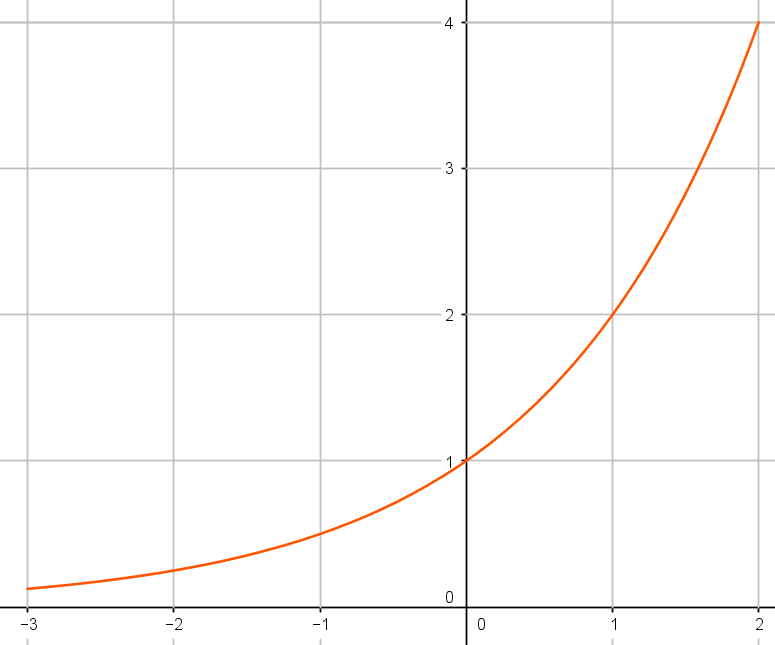
\includegraphics[scale=0.3]{./img/var1}
		\end{center}
		
		\ \\
		$g(x)= 0,5^x$, $0,5 > 1$\\
		la fonction $g$ est décroissante
		
		\begin{center}
			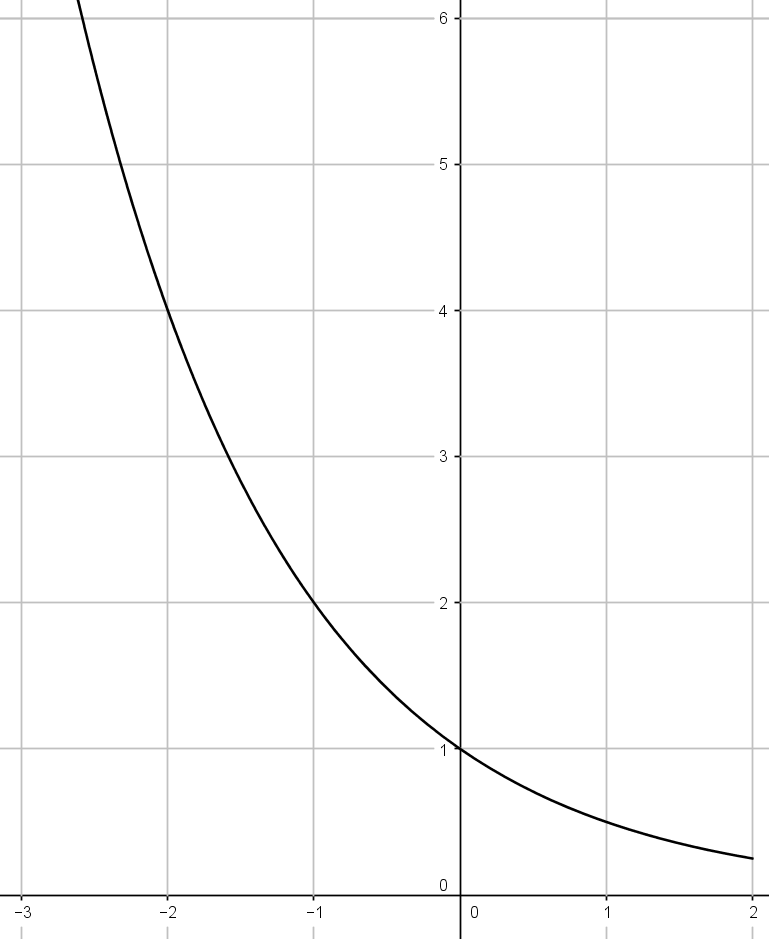
\includegraphics[scale=0.25]{./img/var2}
		\end{center}
	\end{multicols}
\end{myex}

\subsection{Règles de calcul}

\begin{myprops}
	Les règles de calculs sont les mêmes que pour les puissances entières.\\
	$x$ et $y$ sont deux nombres quelconques et $a$ un nombre strictement positif.
	
	\begin{multicols}{2}
		
		\begin{itemize}
			\item $a^x \times a^y = a^{x+y}$
			\item $a^{-x} = \dfrac{1}{a^x}$
			\item $\dfrac{a^x}{a^y} = a^{x-y}$
			%\item $(ab)^x = a^x \times b^x$
			%\item $ \left( \dfrac{a}{b} \right)^x = \dfrac{a^x}{b^x}$
			\item $(a^x)^y = a^{x \times y}$
		\end{itemize}	
		
	\end{multicols}
\end{myprops}

\begin{myexs}
	
	\begin{multicols}{2}
		
	\begin{itemize}
		\item $2^{0.5} \times 2^{1,5} = 2^{0,5 + 1,5} = 2^2 = 4$
		\item $8^{-2} = \dfrac{1}{8^2} = \dfrac{1}{64}$
		\item $\dfrac{5^{5,2}}{5^{2,2}} = 5^{5,2 - 2,2} = 5^3 = 125$
		\item $(10^{0,4})^{5} = 10^{0,4 \times 5} = 10^2 = 100$
	\end{itemize}
	\end{multicols}
\end{myexs}

\newpage

\section{Fonction logarithme décimal}

\subsection{Définition}

\begin{mydef}
	
	Pour tout nombre réel $x$ strictement positif, il existe un unique nombre $a$ tel que $10^a = x$.
	
	
	Ce nombre $a$ est le \kw{logarithme décimal} de $x$, noté $\log(x)$.\\
	
	On a donc :
	\begin{equation*}
		\log(x) = a \Leftrightarrow x = 10^a
	\end{equation*}
		
	La \kw{fonction logarithme décimal} est la fonction $f$, telle que $f(x)=\log(x)$.
\end{mydef}

\subsection{Propriétés et variations}

\begin{myprops}
	\begin{enumerate}
		\item Propriétés :
			\begin{itemize}
				\item Pour tout nombre réel $a$ : $\log(10^a) = a$
				\item Pour tous nombre réels positifs $a$ et $b$ : $\log(a) = \log(b) \Leftrightarrow  a = b$
				\item Pour tous nombre réels positifs $\log (a) < \log (b) \Leftrightarrow a < b $
			\end{itemize}
		\item Valeurs particulières :
			\begin{itemize}
				\item $\log 1 = 0 $
				\item $\log 10 = 1$
				\item $\log 100 = 2$
			\end{itemize}
	
		\item Signe et variations :
			\begin{center}
				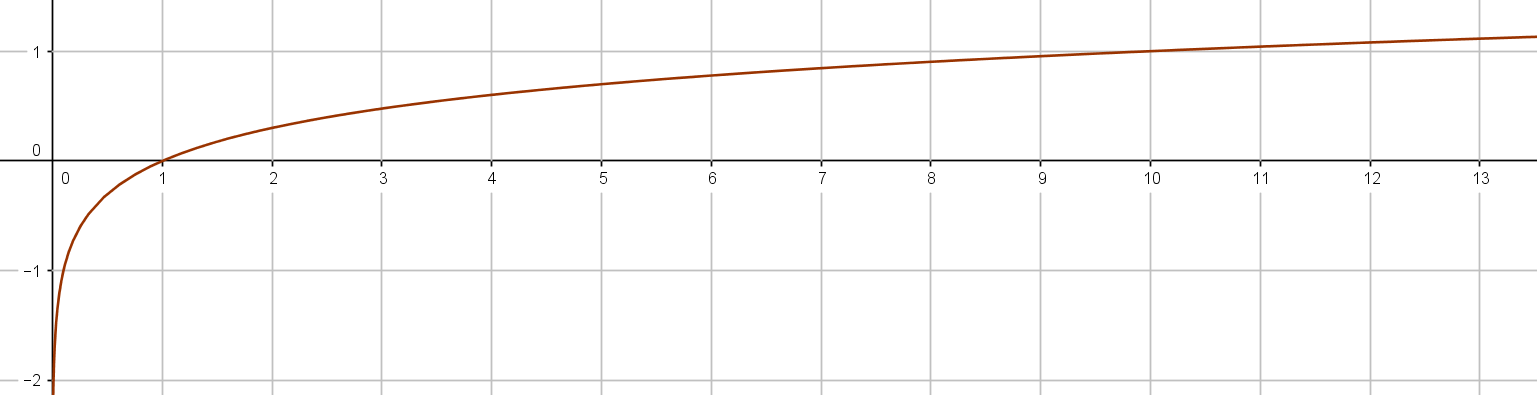
\includegraphics[scale = 0.35]{./img/var_log}
			\end{center}
		
			\begin{multicols}{2}
				\begin{itemize}
				\item La fonction $\log (x)$ est \kw{croissante} pour $x > 0$.			
			
				\item Si $0 \leq x < 1$, alors $\log (x) \leq 0$ .
				
				\item Si $x \geq 1$, alors $\log (x) \geq 0$.	
			\end{itemize}
			 
			\begin{center}
			
			\vspace*{0.5cm}
				
			\begin{variations}
				x & 0 & & 1 & & \pI \\
				\filet
				\log(x) & \bb & - &\z & \dr+ \\				
			\end{variations}
			\end{center}
			\end{multicols}
			 
				
	\end{enumerate}
	
	
\end{myprops}

\subsection{Règles de calcul}

\begin{myprops}
	$a$ et $b$ sont deux nombres strictement positifs :
	
	\begin{multicols}{2}
		\begin{itemize}
			
			\item $\log (a \times b) = \log (a) + \log (b) $
			\item $\log  \left( \dfrac{a}{b} \right) = \log (a) - \log (b) $
			\item $\log(a^x) = x \times log (a) $

	\end{itemize}
	\end{multicols}
\end{myprops}

\section{Résolutions d'\'equations et d'inéquations}

\subsection{\'Equations du type $a^x=b$}

\begin{myex}
	Résoudre l'équation $\num{1.3}^x = 2$ :
	
	\begin{eqnarray*}
		\num{1.3}^x &=& 2 \\
		\log(\num{1.3}^x) &=& \log(2) \\
		x \times \log(\num{1.3}) &=& \log(2) \\
		x &=& \dfrac{\log(2)}{\log(\num{1.3})}\\
	\end{eqnarray*}

\textbf{La solution est donc $\dfrac{\log(2)}{\log(\num{1.3})}$, soit \kw{environ \num{2.64}}.}
\end{myex}

\subsection{Inéquations du type $a^x<b$ et $a^x>b$}

\begin{myex}
	Déterminer les nombres entiers $n$ tels que $4^n \leq 200$. On résout l'équation $4^x \leq 200$ :
	
	
	\begin{eqnarray*}
		4^x &\leq& 200 \\
		\log (4^x) &\leq& \log (200) \\
		x \log (4) &\leq& \log (200) \\
		x &\leq& \dfrac{\log (200)}{\log (4)}  \\
		& & (car \, \log (4) > 0 \; puisque \; 4 > 1) \\
	\end{eqnarray*}

Or $\dfrac{\log (200)}{\log (4)} \approx \num{3.82}$.

\textbf{Les nombres entiers $n$ cherchés sont donc les entiers inférieurs ou égaux à 3.}
\end{myex}

\begin{myex}
	Déterminer les nombres entiers $n$ tels que $1000  \times \num{0.95}^n < 800$. On résout l'équation $\num{0.95}^x < \dfrac{800}{1000}$ :
	
	
	\begin{eqnarray*}
		\num{0.95}^x &<& \num{0.8} \\
		\log (\num{0.95}^x) &<& \log (\num{0.8}) \\
		x \times \log (\num{0.95}) &<& \log (\num{0.8}) \\
		x &>& \dfrac{\log (\num{0.8})}{\log (\num{0.95})} \\
		& & (car \, \log (\num{0.95} < 0 \; puisque \; 0 < \num{0.95} < 1) 		
	\end{eqnarray*}
	
	Or $\dfrac{\log (\num{0.8})}{\log (\num{0.95})} \approx \num{4.35}$.
	
	\textbf{Les nombres entiers $n$ cherchés sont donc les entiers supérieurs ou égaux à 5.}
\end{myex}
\end{document}